\newpage

\section{Rozpraszanie Ramanowskie w ciękich warstwach}
\subsection{Fonony w materiale}
\textbf{Fonon} -  kwazicząstka, kwant energii drgań sieci krystalicznej. Są dwa rodzaje fononów:
\begin{itemize}
	\item{Fonony akustyczne. Powstają w wyniku drgań jednego rodzaju atomów.}
	\item{Fonony optyczne. Powstają w wyniku drgań różnego rodzaju atomów.}
\end{itemize}
Podział fononów jest uzależniony od kształtu relacji dyspersji w pobliżu k=0. \\
Fonony akustyczne wykazują zależność:
\begin{equation}
	\lim_{k \to 0} \omega(k) = 0
\end{equation}
natomiast fonony optyczne:
\begin{equation}
\lim_{k \to 0} \omega(k) = const
\end{equation}
\begin{figure}[H]
	\begin{center}
		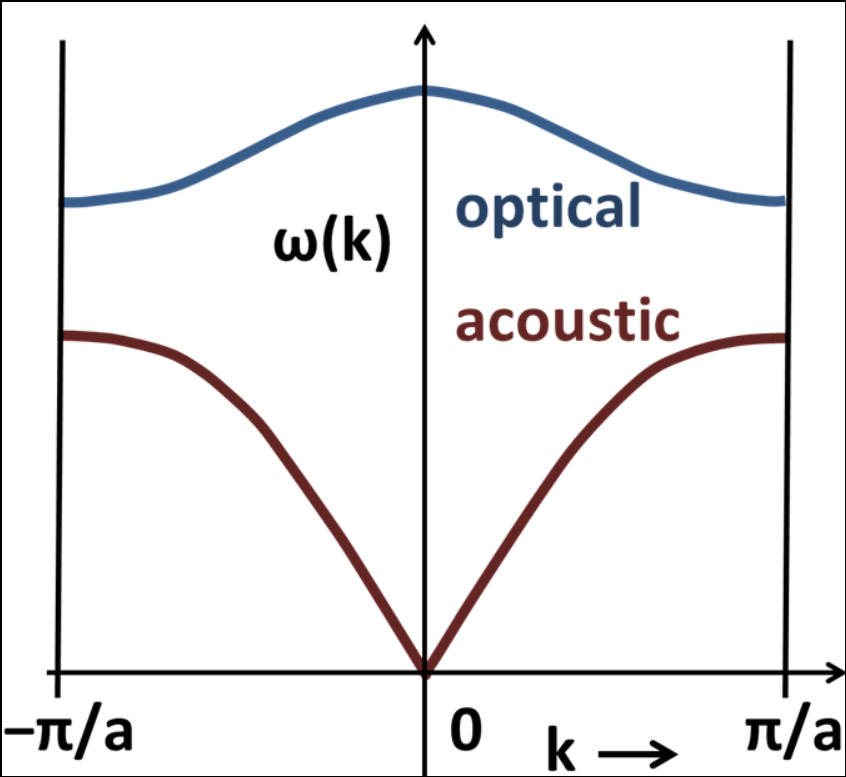
\includegraphics[width=0.8\linewidth]{Rozpraszanie-Ramanowskie-Ciekie/Phonons.png}
		\caption{Krzywe dyspersyjne dla liniowego łańcucha dwuatomowego.[5]}
	\end{center}
\end{figure}
Dla kryształu zawierającego N(>2) różnych atomów w komórce prymitywnej relacja dyspersji zawiera trzy gałęzie akustyczne oraz $\alpha$N-3 gałęzie optyczne, gdzie $\alpha$ to jest wymiar. Więc dla liniowego łańcucha dwuatomowego N=2 mamy jedną gałąź optyczną i jedną akustyczną. A dla trójwymiarowej komórki prostej składającej się z dwóch różnych cząsteczek będą 3 krzywe optyczne i 3 akustyczne.

Przy rozpraszaniu fotonów na fononach powinny być spełnione dwa prawa zachowania: 

Prawo zachowania energii:
\begin{equation}
	\hbar \mathbf{\omega_{i}} = \hbar \mathbf{\omega_{s}} \pm \hbar \mathbf{\Omega_{fonon}}
\end{equation}
\begin{itemize}
	\item $\omega_{i}$ - częstotliwość fotonu padającego;
	\item $\omega_{s}$ - częstotliwość fotonu rozproszonego;
	\item $\Omega_{fonon}$ - częstotliwość fononu;
	\item $\hbar$ - stała Plancka.
\end{itemize}

Prawo zachowania pędu:
\begin{equation}
	\hbar \mathbf{k_{i}} = \hbar \mathbf{k_{s}} \pm \hbar \mathbf{K_{fonon}}
\end{equation}
\begin{itemize}	
	\item $k_{i}$ - wektor falowy fotonu padającego;
	\item $k_{s}$ - wektor falowy fotonu rozproszonego;
	\item $K_{fonon}$ - wektor falowy fononu;
	\item $\hbar$ - stała Plancka.
\end{itemize}

Pęd fononu jest znacznie większy od pędu fotonu, a energia fotonu jest 
znacznie większa od energii fononu. To znaczy że uczęstniczą w oddziaływaniu tylko te 
fonony co mają mały pęd.

\begin{figure}[H]
	\begin{center}
		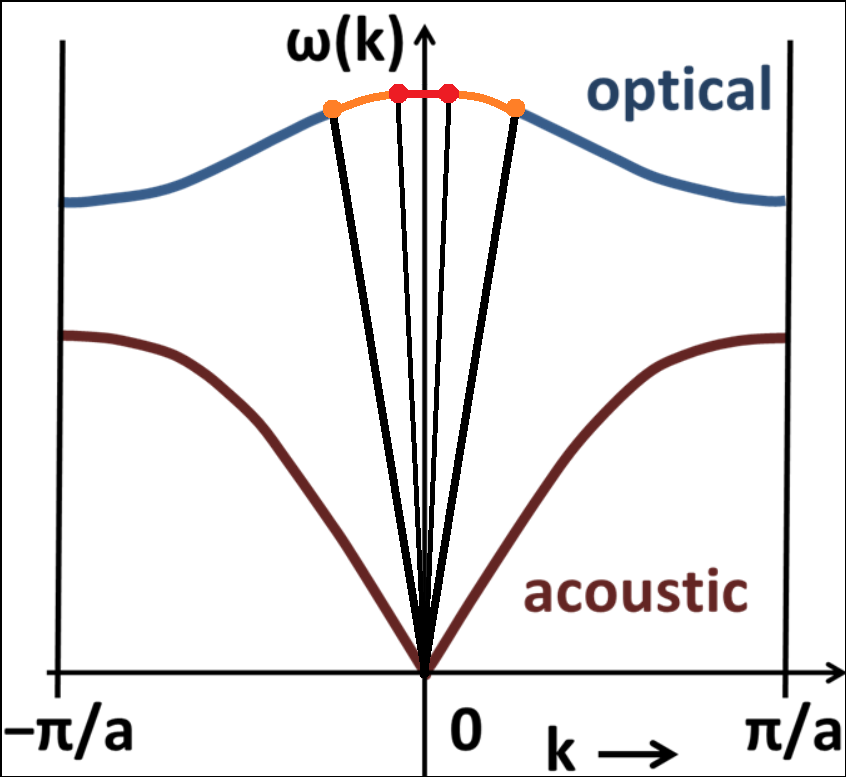
\includegraphics[width=0.8\linewidth]{Rozpraszanie-Ramanowskie-Ciekie/PhononsCenter.png}
		\caption{Krzywe dyspersyjne z zaznaczonym obszarem pokazującym które fonony uczęstniczą w rozpraszaniu ramanowskim.}
	\end{center}
\end{figure}

Z powyższego rysunku widzimy, że w oddziaływaniach przyjmują udział tylko optyczne fonony co znajdują się w środku strefy Brillouina. Akustyczne fonony nie biorą udziału dlatego, że dla $k \rightarrow 0$ energia też dąży do zera.

\vspace{1cm}
W niniejszej pracy były badane tylko widma stokesowskie dla tego, że one są bardziej intensywne niż widma antystokesowskie. Miarą intensywności widma są piki, które uzyskujemy. Im większe piki, tym mniejszy błąd przy analizie wyników pomiaru.
Prawdopodobieństwo obsadzenia stanu energetycznego fononem jest proporcjonalne do:
\begin{equation}
	\sim \exp^{-\frac{E}{kT}} 
\end{equation}
\begin{itemize}
	\item{$E$ - energia stanu energicznego};
	\item{$k$ - stała Boltzmanna};
	\item{$T$ - temperatura w Kelwinach}.
\end{itemize}
to znaczy że stosunek intensywności promieniowania rozproszonego w widmie antystokesowskim
do intensywności promieniowania pobudzającego jest:
\begin{equation}
	\frac{I_{ants}}{I} \sim \exp^{-\frac{E}{kT}}
\end{equation}
\begin{itemize}
	\item{$I_{ants}$ - intensywność promieniowania w widmie antystokesowskim};
	\item{$I$ - intensywność promieniowania pobudzającego}
\end{itemize}
	Typowa energia wzbudzenia fononu $E = 0.065eV$, więc:
\begin{equation}
	\sim \exp^{-\frac{E}{kT}} = \exp^{-\frac{0.065}{0.025}} \approx 0.07
\end{equation}
Czyli intensywność widma antystokesowskiego wynosi $7\%$ widma stokesowskiego. 
\subsection{Co można odczytać z widma Ramanowskiego}
Ważną rolę w widmie Ramanowskim odgrywa szerokość połówkowa pików.
Na podstawie informacji o szerokości połówkowej $\Gamma$ można mówić o czasie życia fononów w próbce:
\begin{equation}
	\Gamma \sim \frac{1}{\tau}
\end{equation}

gdzie $\tau$ - czas życia fononu.

\begin{figure}[H]
	\begin{center}
		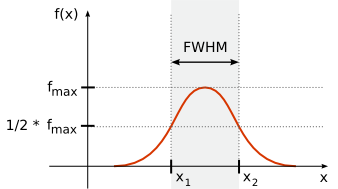
\includegraphics[width=0.8\linewidth]{Full_width_at_half_maximum.png}
		\caption{Szerokość połówkowa piku \textit{FWHM} - z angielskiego \textit{Full Width at Half Maximum}.}
	\end{center}
\end{figure}

Szerokość połówkowa zależy od:
\begin{itemize}
	\item[1]{Rozmiar próbki. Czy materiał jest cienkowarstwowym, czy bulk.}
	\item[2]{Defekty. Fonony rozpraszają się na defektach, co zmniejsza czas ich życia.}
	\item[3]{Rozpraszanie fononów wskutek efektów anharmonicznych}
\end{itemize}
Na podstawie szerokości piku można uzyskać informację o przewodnictwie cieplnym próbki. 
W zależności od ilości i kształtu pików można zbadać jaki to jest materiał, czy badany materiał jest czystym materiałem bez domieszek.
Na podstawie widma Ramanowskiego można oszacować temperaturę ciała. Czyli jest możliwy pomiar temperatury bez ingeracji do badanego materiału.

\subsection{Piki ramanowskie w cienkich warstwach}
W materiałach cienkowarstwowych jeden z wymiarów jest rzędu kilku nanometrów. To powoduje że zaczynają odgrywać ważną rolę efekty kwantowe. Z zasady nieoznaczoności Heisenberga:
\begin{equation}
	\Delta p_{fon} \Delta d \geq \frac{\hbar}{2}
\end{equation}
\begin{itemize}
	\item{$\Delta p_{fon}$ - niepewność pomiaru pędu fononu};
	\item{$\Delta d$ - niepewność pomiaru położenia fononu}
\end{itemize}
Mniejsza niepewność położenia fononu powoduje większą niepewność pędu fononu. To znaczy że w rozpraszaniu ramanowskim będą uczęstniczyć optyczne fonony o mniejszej energii, które są z większego zakresu energii ze środka strefy Brillouine'a.

\begin{figure}[H]
	\begin{center}
		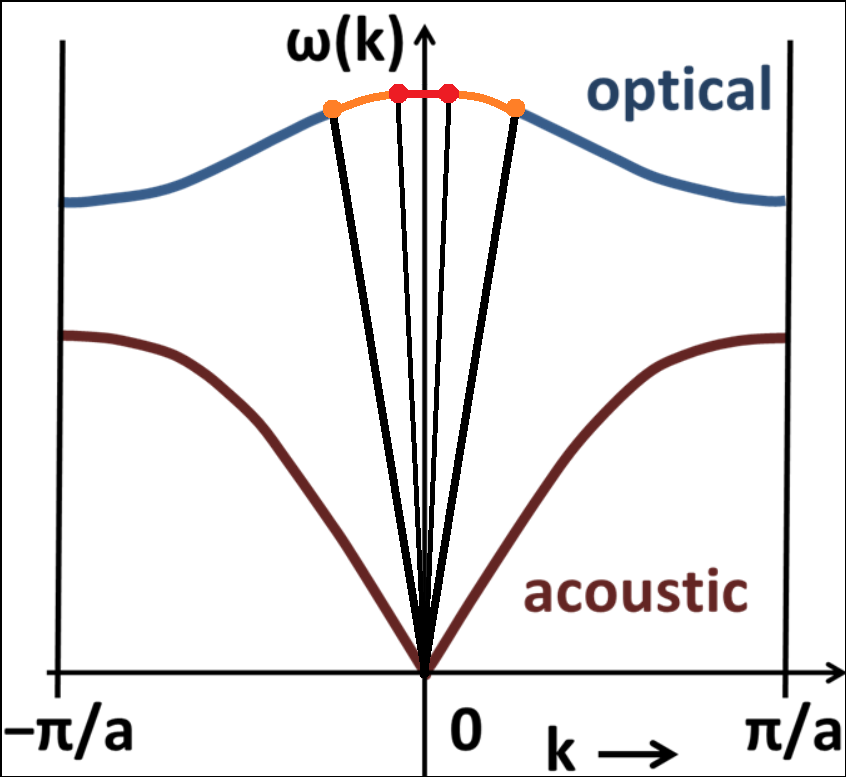
\includegraphics[width=0.8\linewidth]{Rozpraszanie-Ramanowskie-Ciekie/PhononsCenterQuantum.png}
		\caption{Krzywe dyspersyjne z zaznaczonym obszarem pokazującym które fonony uczęstniczą w rozpraszaniu ramanowskim w ciękich warstwach.}
	\end{center}
\end{figure}

Taka rozbieżność w energii wpływa na kształt powstających pików w widmie ramanowskim.
Piki są przesunięte w kierunku mniejszej energii i p stronie mniejszych energii są wydłużone.

\begin{figure}[H]
	\begin{center}
		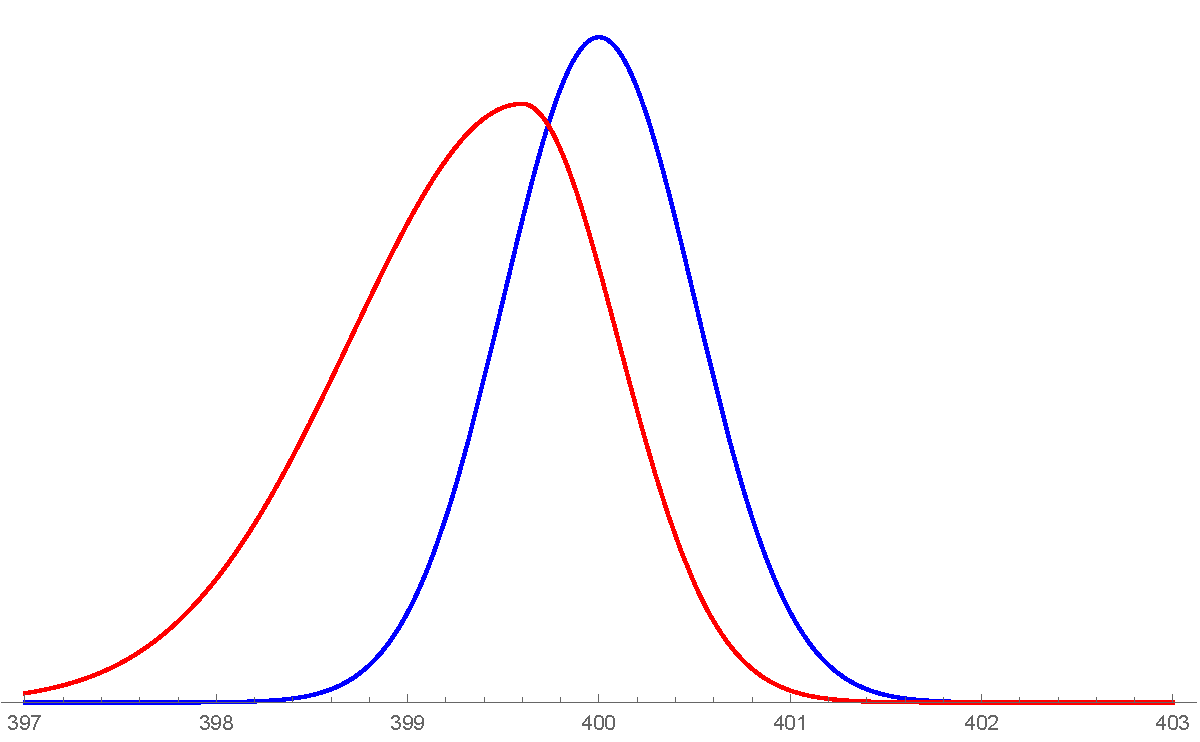
\includegraphics[width=0.8\linewidth]{Rozpraszanie-Ramanowskie-Ciekie/piki.pdf}
		\caption{Kształt piku widma ramanowskiego dla cienkich warstw.}
	\end{center}
\end{figure}

Napisać o rozpraszaniu dwufononowym

\subsection{Dane dla pików ramanowskich GaP Ga2S3}

\subsection{przyrząd pomiarowy, rysunek, opis}
